\documentclass{standalone}
\usepackage{tikz}
\begin{document}
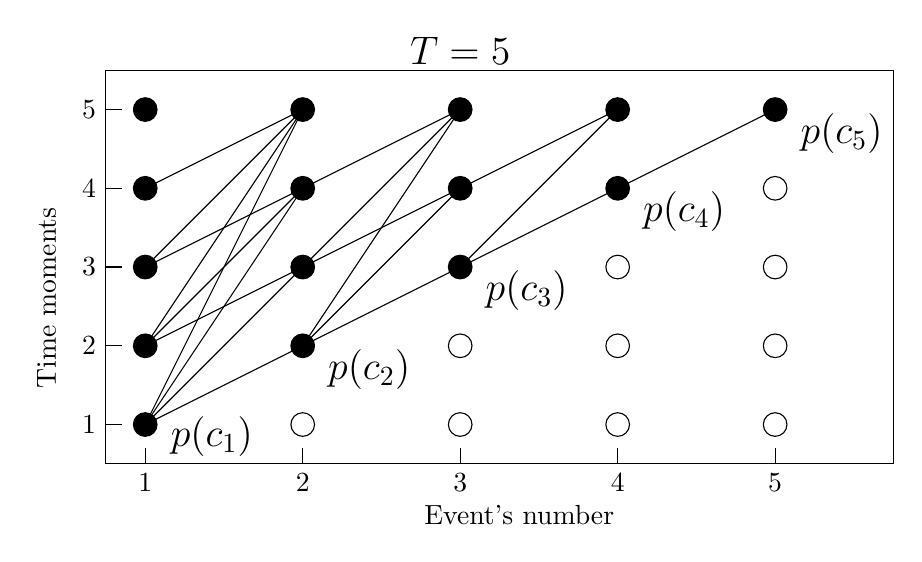
\begin{tikzpicture}[scale=1.0, yscale = 1.0, xscale = 1.0]
\def\xstep{2.0}
\def\ystep{1.0}
\def\rad{0.15}
\def\ticksz{0.2};
\def\recheight{4.5};
\def\recwidth{9.5};
\draw [black] (-0.5, -0.5) rectangle (\recwidth,\recheight);
\node at (4.0, \recheight + 0.25) {\Large $T=5$};
%\node at (-1.3, \recheight + 0.5) {\Large $w=3$};
%\node [below, rotate=90] at (-1.5, \recheight/2 - \recheight/7) {\Large Y: Time};
\node [below, rotate=90] at (-1.5, \recheight/2 - \recheight/7) {Time moments};
%\node [below] at (\recwidth, -0.5) {\Large $i$};
%\node [below] at (\recwidth/2, -0.9) {\Large X: Event's number, $i$};
\node [below] at (\recwidth/2, -0.9) {Event's number};
%\draw ( - 0.2, - 0.3) rectangle ( 0.2, 2 + 0.3);
%\draw (2 - 0.2, 1 - 0.3) rectangle (2 + 0.2, 5 + 0.3);
%\draw (4-0.2, 6.5) -- (4-0.2, 2-0.3) -- (4+0.2, 2-0.3) -- (4+0.2, 6.5) ;
\node[right] at (0.2, -0.15)   {\Large $p(c_1)$};
\node[right] at (2+0.2,1 -0.3) {\Large $p(c_2)$};
\node[right] at (4+0.2, 2-0.3) {\Large $p(c_3)$};
\node[right] at (6+0.2, 3-0.3) {\Large $p(c_4)$};
\node[right] at (8+0.2, 4-0.3) {\Large $p(c_5)$};
%
%%%%%%%%%%%%%%%%%%%%%%%%%%%
%%%%%%%%%%%% 1 %%%%%%%%%%%%
\draw[fill=black] (0, 0       ) circle (\rad);
\draw[fill=black] (0, 1*\ystep) circle (\rad);
\draw[fill=black] (0, 2*\ystep) circle (\rad);
\draw[fill=black] (0, 3*\ystep) circle (\rad);
\draw[fill=black] (0, 4*\ystep) circle (\rad);
%\draw[fill=black] (0, 5*\ystep) circle (\rad);
%\draw[fill=black] (0, 6*\ystep) circle (\rad);
% x-Tick 1
\draw (0, - 0.5) -- (0, - 0.5 + \ticksz);
\node [below] at (0, - 0.5) {$1$};
% y-Tick 1
\draw (-0.5, 0*\ystep) -- (-0.5 + \ticksz, 0*\ystep);
\node [left] at (-0.5, 0*\ystep) {$1$};
% Line from node (1,1)
\draw (0, 0) -- (\xstep, 1*\ystep);
\draw (0, 0) -- (\xstep, 2*\ystep);
\draw (0, 0) -- (\xstep, 3*\ystep);
\draw (0, 0) -- (\xstep, 4*\ystep);
% Line from node (1,2)
\draw (0, \ystep) -- (\xstep, 2*\ystep);
\draw (0, \ystep) -- (\xstep, 3*\ystep);
\draw (0, \ystep) -- (\xstep, 4*\ystep);
% Line from node (1,3)
\draw (0, 2*\ystep) -- (\xstep, 3*\ystep);
\draw (0, 2*\ystep) -- (\xstep, 4*\ystep);
%\draw (0, 2*\ystep) -- (\xstep, 5*\ystep);
% Line from node (1,4)
\draw (0, 3*\ystep) -- (\xstep, 4*\ystep);
%%%%%%%%%%%%%%%%%%%%%%%%%%%
%%%%%%%%%%%% 2 %%%%%%%%%%%%
\draw[fill=white] (\xstep, 0       ) circle (\rad);
\draw[fill=black] (\xstep, 1*\ystep) circle (\rad);
\draw[fill=black] (\xstep, 2*\ystep) circle (\rad);
\draw[fill=black] (\xstep, 3*\ystep) circle (\rad);
\draw[fill=black] (\xstep, 4*\ystep) circle (\rad);
%\draw[fill=black] (\xstep, 5*\ystep) circle (\rad);
%\draw[fill=white] (\xstep, 6*\ystep) circle (\rad);
% x-Tick 2
\draw (\xstep, - 0.5) -- (\xstep, - 0.5 + \ticksz);
\node [below] at (\xstep, - 0.5) {$2$};
% y-Ticks 2
\draw (-0.5, 1*\ystep) -- (-0.5 + \ticksz, 1*\ystep);
%\draw (-0.5, 5*\ystep) -- (-0.5 + \ticksz, 5*\ystep);
%\draw (-0.5, 6*\ystep) -- (-0.5 + \ticksz, 6*\ystep);
\node [left] at (-0.5, 1*\ystep) {$2$};
% Line from node (2,1)
\draw (\xstep, 1*\ystep) -- (2*\xstep, 2*\ystep);
\draw (\xstep, 1*\ystep) -- (2*\xstep, 3*\ystep);
\draw (\xstep, 1*\ystep) -- (2*\xstep, 4*\ystep);
% Line from node (2,2)
\draw (\xstep, 2*\ystep) -- (2*\xstep, 3*\ystep);
\draw (\xstep, 2*\ystep) -- (2*\xstep, 4*\ystep);
%\draw[dashed] (\xstep, 2*\ystep) -- (2*\xstep, 5*\ystep);
% Line from node (2,3)
\draw (\xstep, 3*\ystep) -- (2*\xstep, 4*\ystep);
%\draw[dashed] (\xstep, 3*\ystep) -- (2*\xstep, 5*\ystep);
%\draw[dashed] (\xstep, 3*\ystep) -- (2*\xstep, 6*\ystep);
%%%%%%%%%%%%%%%%%%%%%%%%%%%
%%%%%%%%%%%% 3 %%%%%%%%%%%%
\draw[fill=white] (2*\xstep, 0       ) circle (\rad);
\draw[fill=white] (2*\xstep, 1*\ystep) circle (\rad);
\draw[fill=black] (2*\xstep, 2*\ystep) circle (\rad);
\draw[fill=black] (2*\xstep, 3*\ystep) circle (\rad);
\draw[fill=black] (2*\xstep, 4*\ystep) circle (\rad);
% Line from node (3,1)
\draw (2*\xstep, 2*\ystep) -- (3*\xstep, 3*\ystep);
% Line from node (3,2)
\draw (2*\xstep, 2*\ystep) -- (3*\xstep, 4*\ystep);
\draw (2*\xstep, 3*\ystep) -- (3*\xstep, 4*\ystep);
% Line from node (4,5)
\draw (3*\xstep, 3*\ystep) -- (4*\xstep, 4*\ystep);
% x-Tick 3
\draw (2*\xstep, - 0.5) -- (2*\xstep, - 0.5 + \ticksz);
\node [below] at (2*\xstep, - 0.5) {$3$};
% x-Tick 4
\draw (3*\xstep, - 0.5) -- (3*\xstep, - 0.5 + \ticksz);
\node [below] at (3*\xstep, - 0.5) {$4$};
% x-Tick 5
\draw (4*\xstep, - 0.5) -- (4*\xstep, - 0.5 + \ticksz);
\node [below] at (4*\xstep, - 0.5) {$5$};
% y-Tick 3
\draw (-0.5, 2*\ystep) -- (-0.5 + \ticksz, 2*\ystep);
\node [left] at (-0.5, 2*\ystep) {$3$};
% y-Tick 4
\draw (-0.5, 3*\ystep) -- (-0.5 + \ticksz, 3*\ystep);
\node [left] at (-0.5, 3*\ystep) {$4$};
% y-Tick 5
\draw (-0.5, 4*\ystep) -- (-0.5 + \ticksz, 4*\ystep);
\node [left] at (-0.5, 4*\ystep) {$5$};
%\node [left] at (-0.5, 5*\ystep) {$6$};
%\node [left] at (-0.5, 6*\ystep) {$7$};
%%%%%%%%%%%%%%%%%%%%%%%%%%%
%%%%%%%%%%%% 4 %%%%%%%%%%%%
\draw[fill=white] (3*\xstep, 0       ) circle (\rad);
\draw[fill=white] (3*\xstep, 1*\ystep) circle (\rad);
\draw[fill=white] (3*\xstep, 2*\ystep) circle (\rad);
\draw[fill=black] (3*\xstep, 3*\ystep) circle (\rad);
\draw[fill=black] (3*\xstep, 4*\ystep) circle (\rad);
%%%%%%%%%%%%%%%%%%%%%%%%%%%
%%%%%%%%%%%% 5 %%%%%%%%%%%%
\draw[fill=white] (4*\xstep, 0       ) circle (\rad);
\draw[fill=white] (4*\xstep, 1*\ystep) circle (\rad);
\draw[fill=white] (4*\xstep, 2*\ystep) circle (\rad);
\draw[fill=white] (4*\xstep, 3*\ystep) circle (\rad);
\draw[fill=black] (4*\xstep, 4*\ystep) circle (\rad);
\end{tikzpicture}
\end{document}